\section{センサーボードを使ってみよう}
\subsection{センサーボードって何だろう}

センサーボードとは、ラズベリーパイの上部に接続することでラズベリーパイで出来ることを拡張するための基板です。子ども IT 未来塾では Indoor Corgi Elec. という会社が販売している RPZ-IR-Sensor を使います。下記 URL から販売ページを見ることができます。これを使うことで、例えばスイッチを使ったり、温度や湿度を計測したり、赤外線で動く家電を操作したりすることができるようになります。\\
\url{https://www.indoorcorgielec.com/products/rpz-ir-sensor/}\\

\begin{figure}[H]
    \centering
    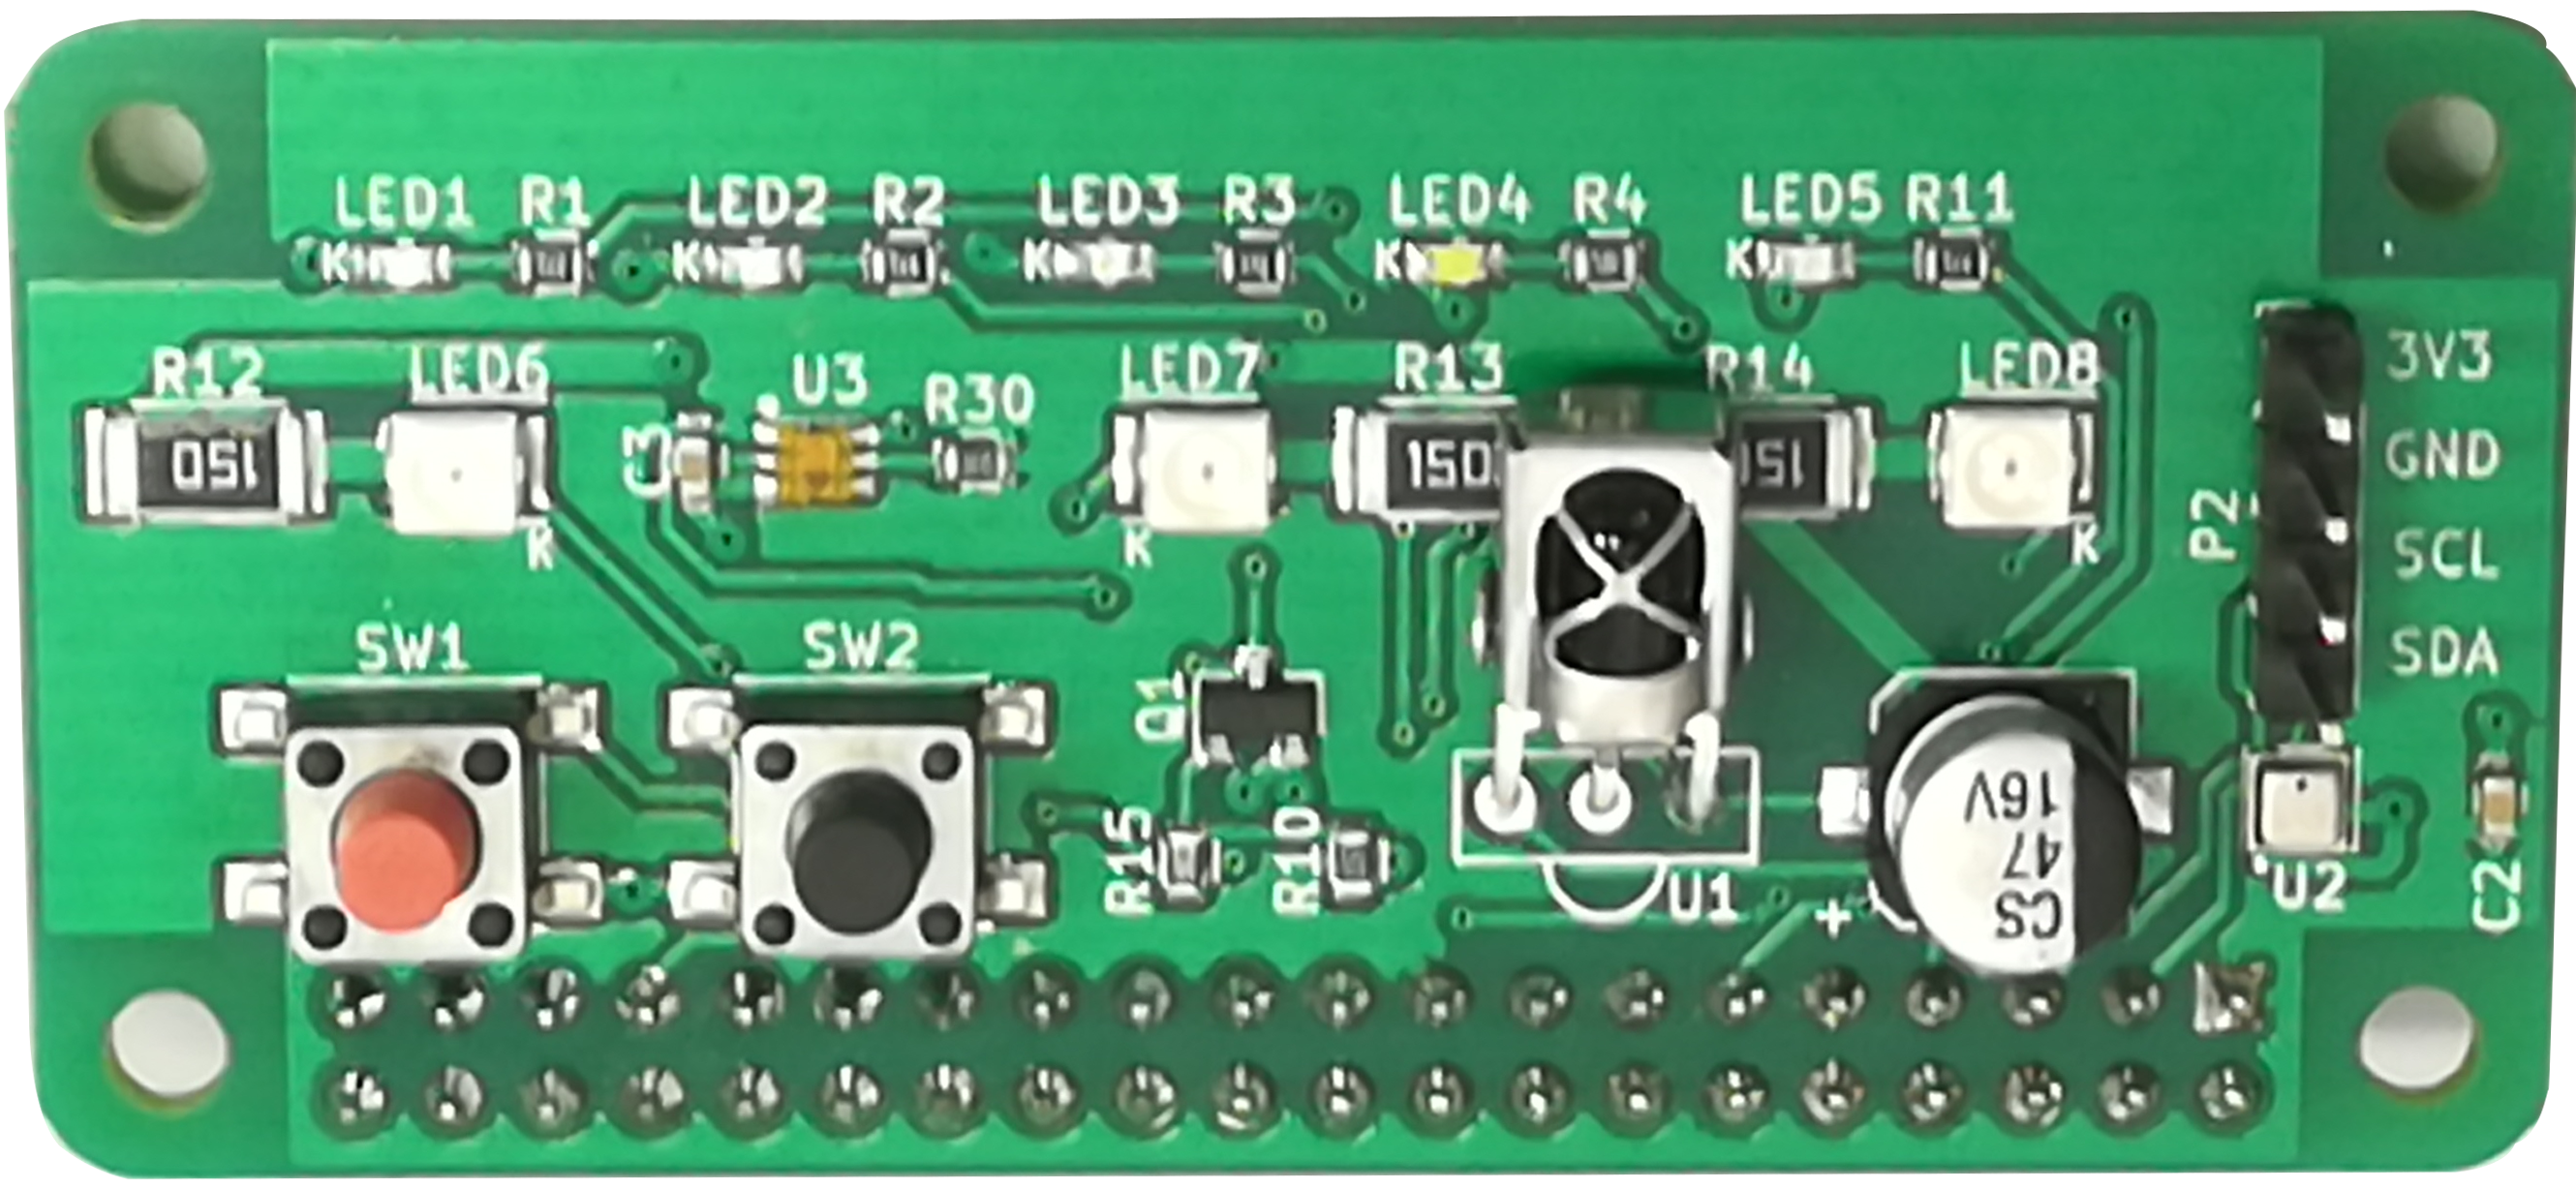
\includegraphics[width=0.6\linewidth]{images/chap03/text03-img030.png}
    \caption{センサーボード}
\end{figure}

温湿度気圧センサーはセンサーボード上に取り付けられたセンサーと、外付けのセンサーの2種類があります。センサーボード上のセンサーがラズベリーパイの熱のせいで熱くなってしまうので、基本的には外付けのセンサーを使いましょう。

外付けセンサーを取り付けるときはピンに正しい向きがあるので、赤い線が3V3にささるように、下の写真のように取り付けてください。

\begin{figure}[H]
    \centering
    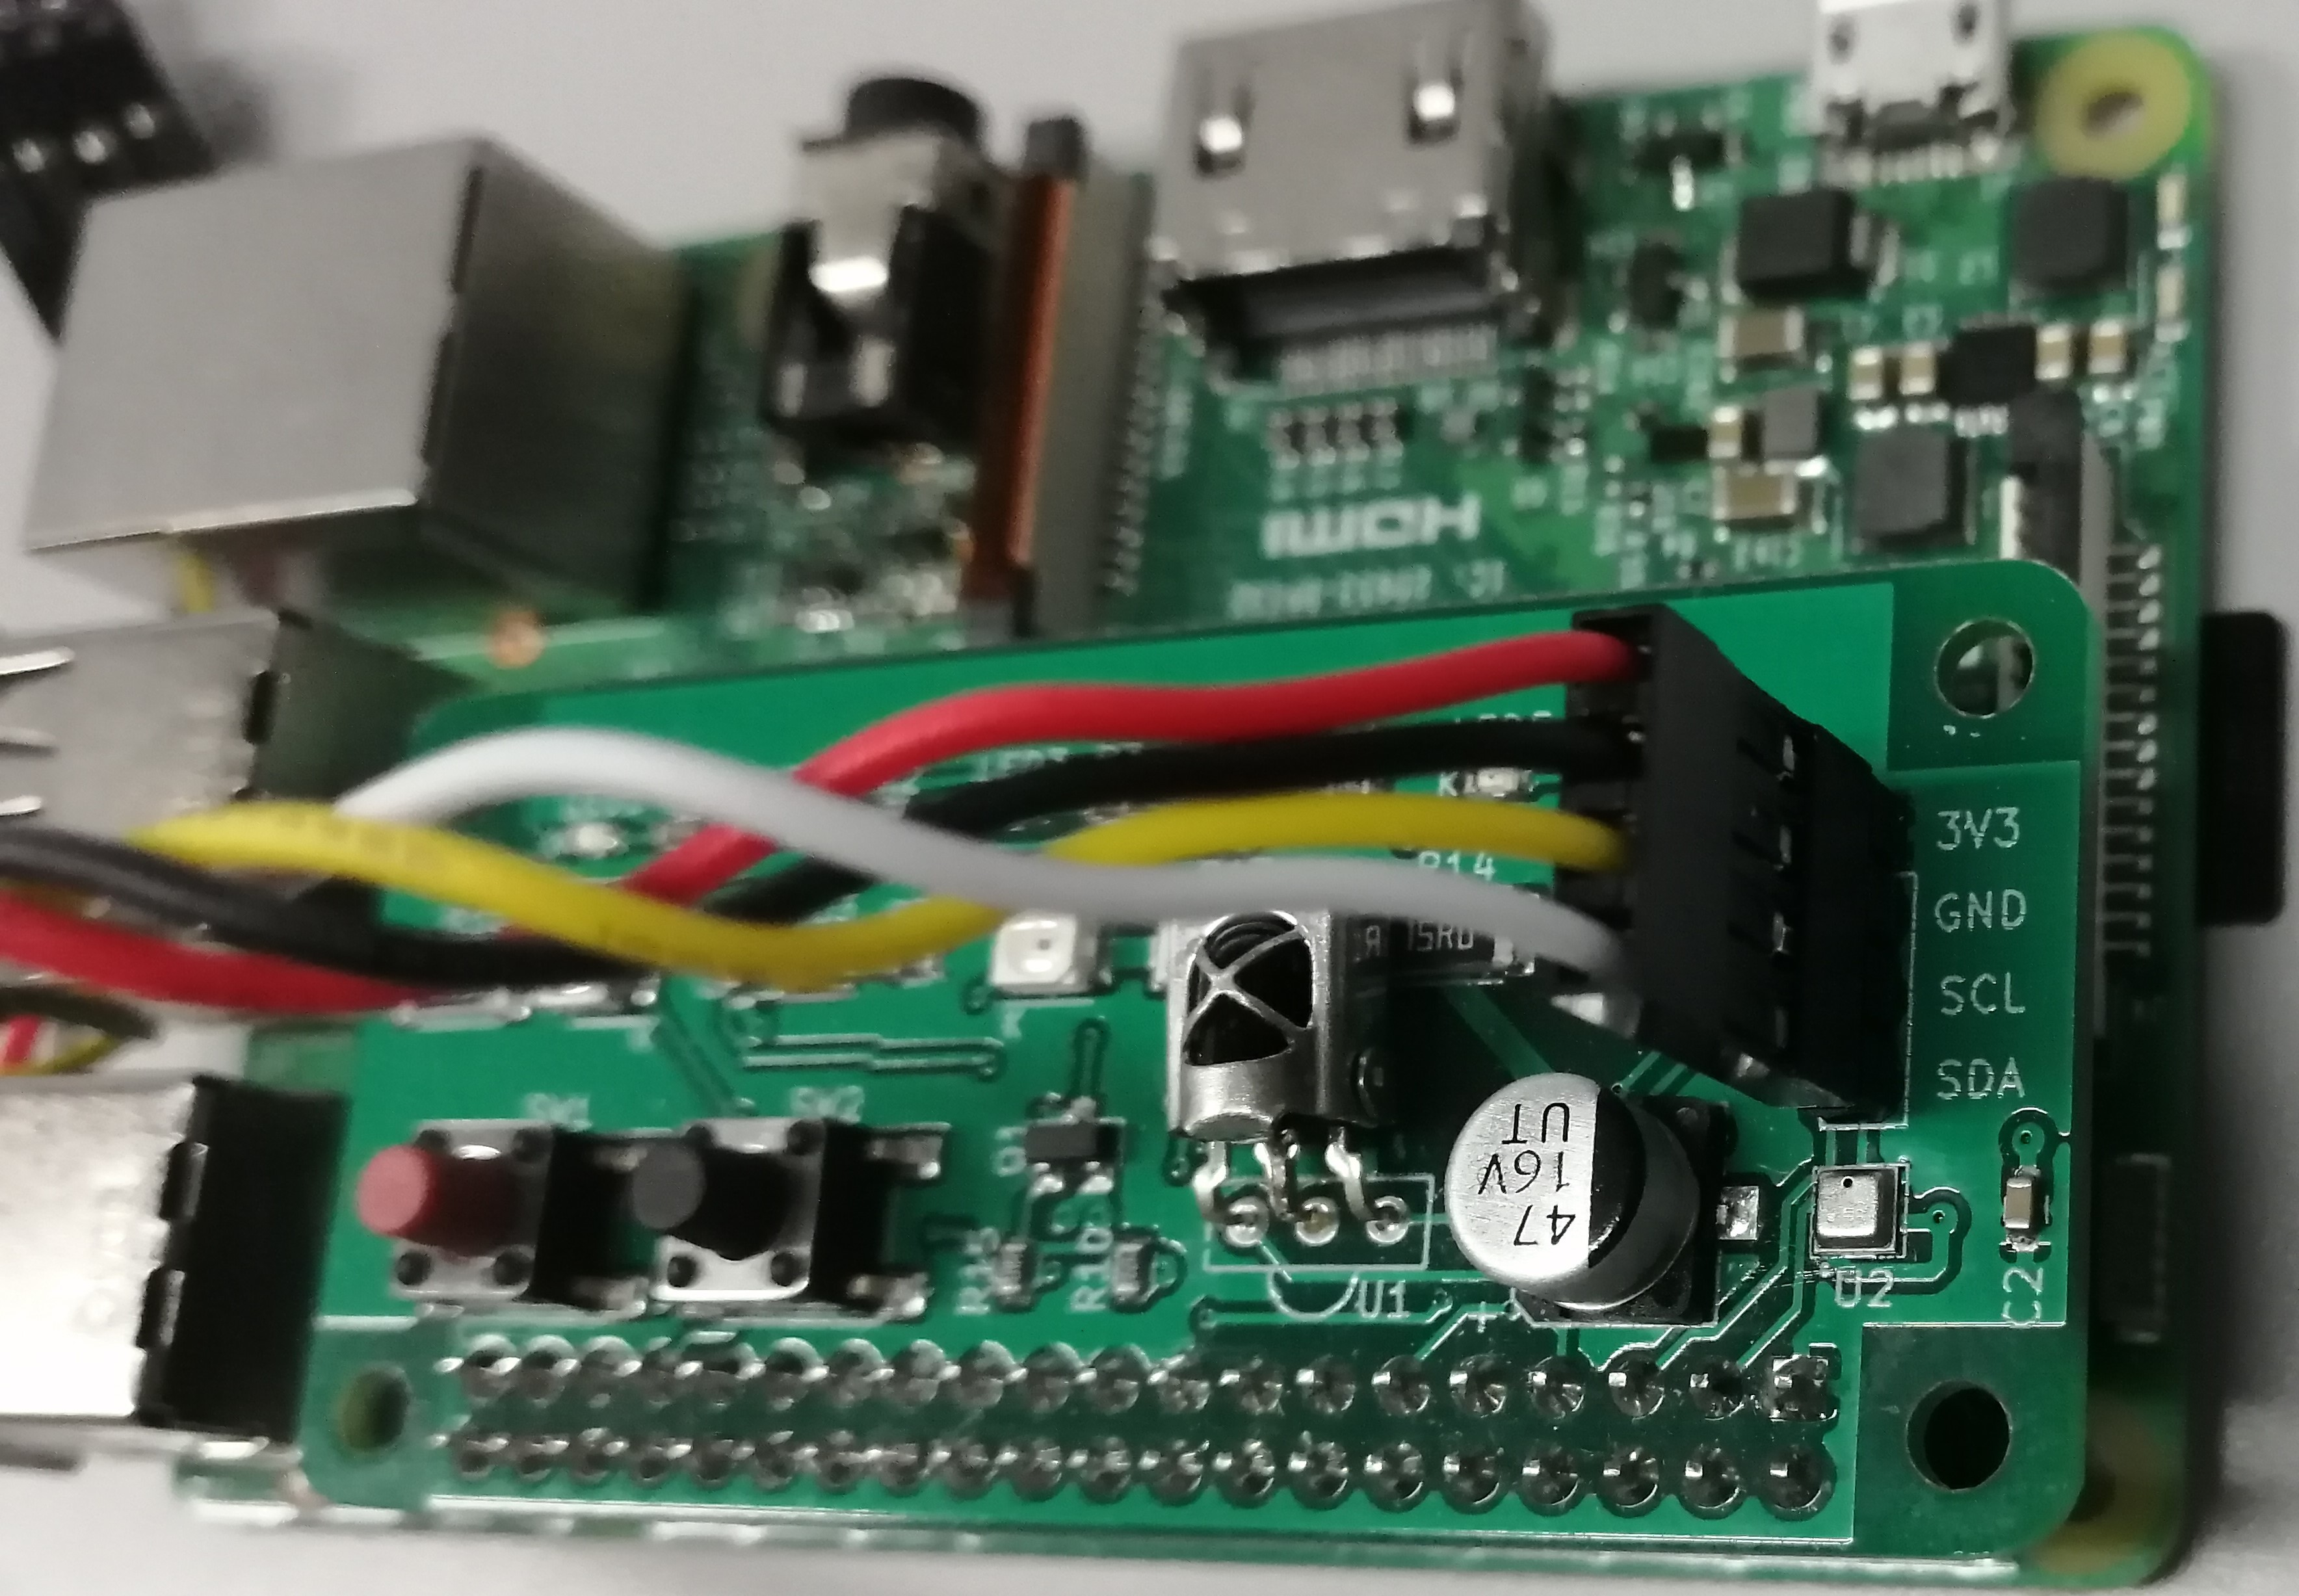
\includegraphics[width=0.6\linewidth]{images/chap03/text03-img034.jpg}
    \caption{外付けセンサーの取り付け方法}
\end{figure}

センサーボードとラズベリーパイは図\ref{sensors}のように接続されています。たとえば LED1 を使いたいときは GPIO17 というピンを使います。

\begin{figure}[H]
    \centering
    \includesvg[width=\linewidth]{images/chap03/rpz-ir-sensor.svg}
    \caption{センサーボードとラズベリーパイのかんけい}
    \label{sensors}
\end{figure}

\section{LEDの点灯・消灯を制御してみよう}
\subsection{LED を光らせよう}

まずはセンサーボードにある LED を光らせてみましょう。HSP スクリプトエディタから LED を光らせるプログラム(led.hsp)を読み込んで実行してみましょう。led.hsp は、\textasciitilde /03のディレクトリにあります。\\

\begin{lstlisting}[caption=led.hsp,label=led.hsp]
#include "hsp3dish.as"		<#blue#;スクリプトの設定を読み込む#>
#include "rpz-gpio.as"		<#blue#;スクリプトの設定を読み込む#>
	redraw 0		<#blue#;画面更新(仮想画面に描画)#>
	font "",30		<#blue#;文字のフォント、サイズを決める#>
	pos 20,20		<#blue#;文字の場所を決める#>
	mes "LED が光るよ"	<#blue#;文字を決める#>
	redraw 1		<#blue#;画面更新(実際の画面に描画)#>
*led
	gpio 17, 1		<#blue#;GPIO17 を点灯させる#>
	await 100		<#blue#;0.1 秒待つ#>
	goto *led		<#blue#;*led まで戻る#>
	gpio 17, 0		<#blue#;GPIO17を消灯させる#>
\end{lstlisting}

下の写真のように LED が光りましたか?\\

\begin{figure}[H]
    \centering
    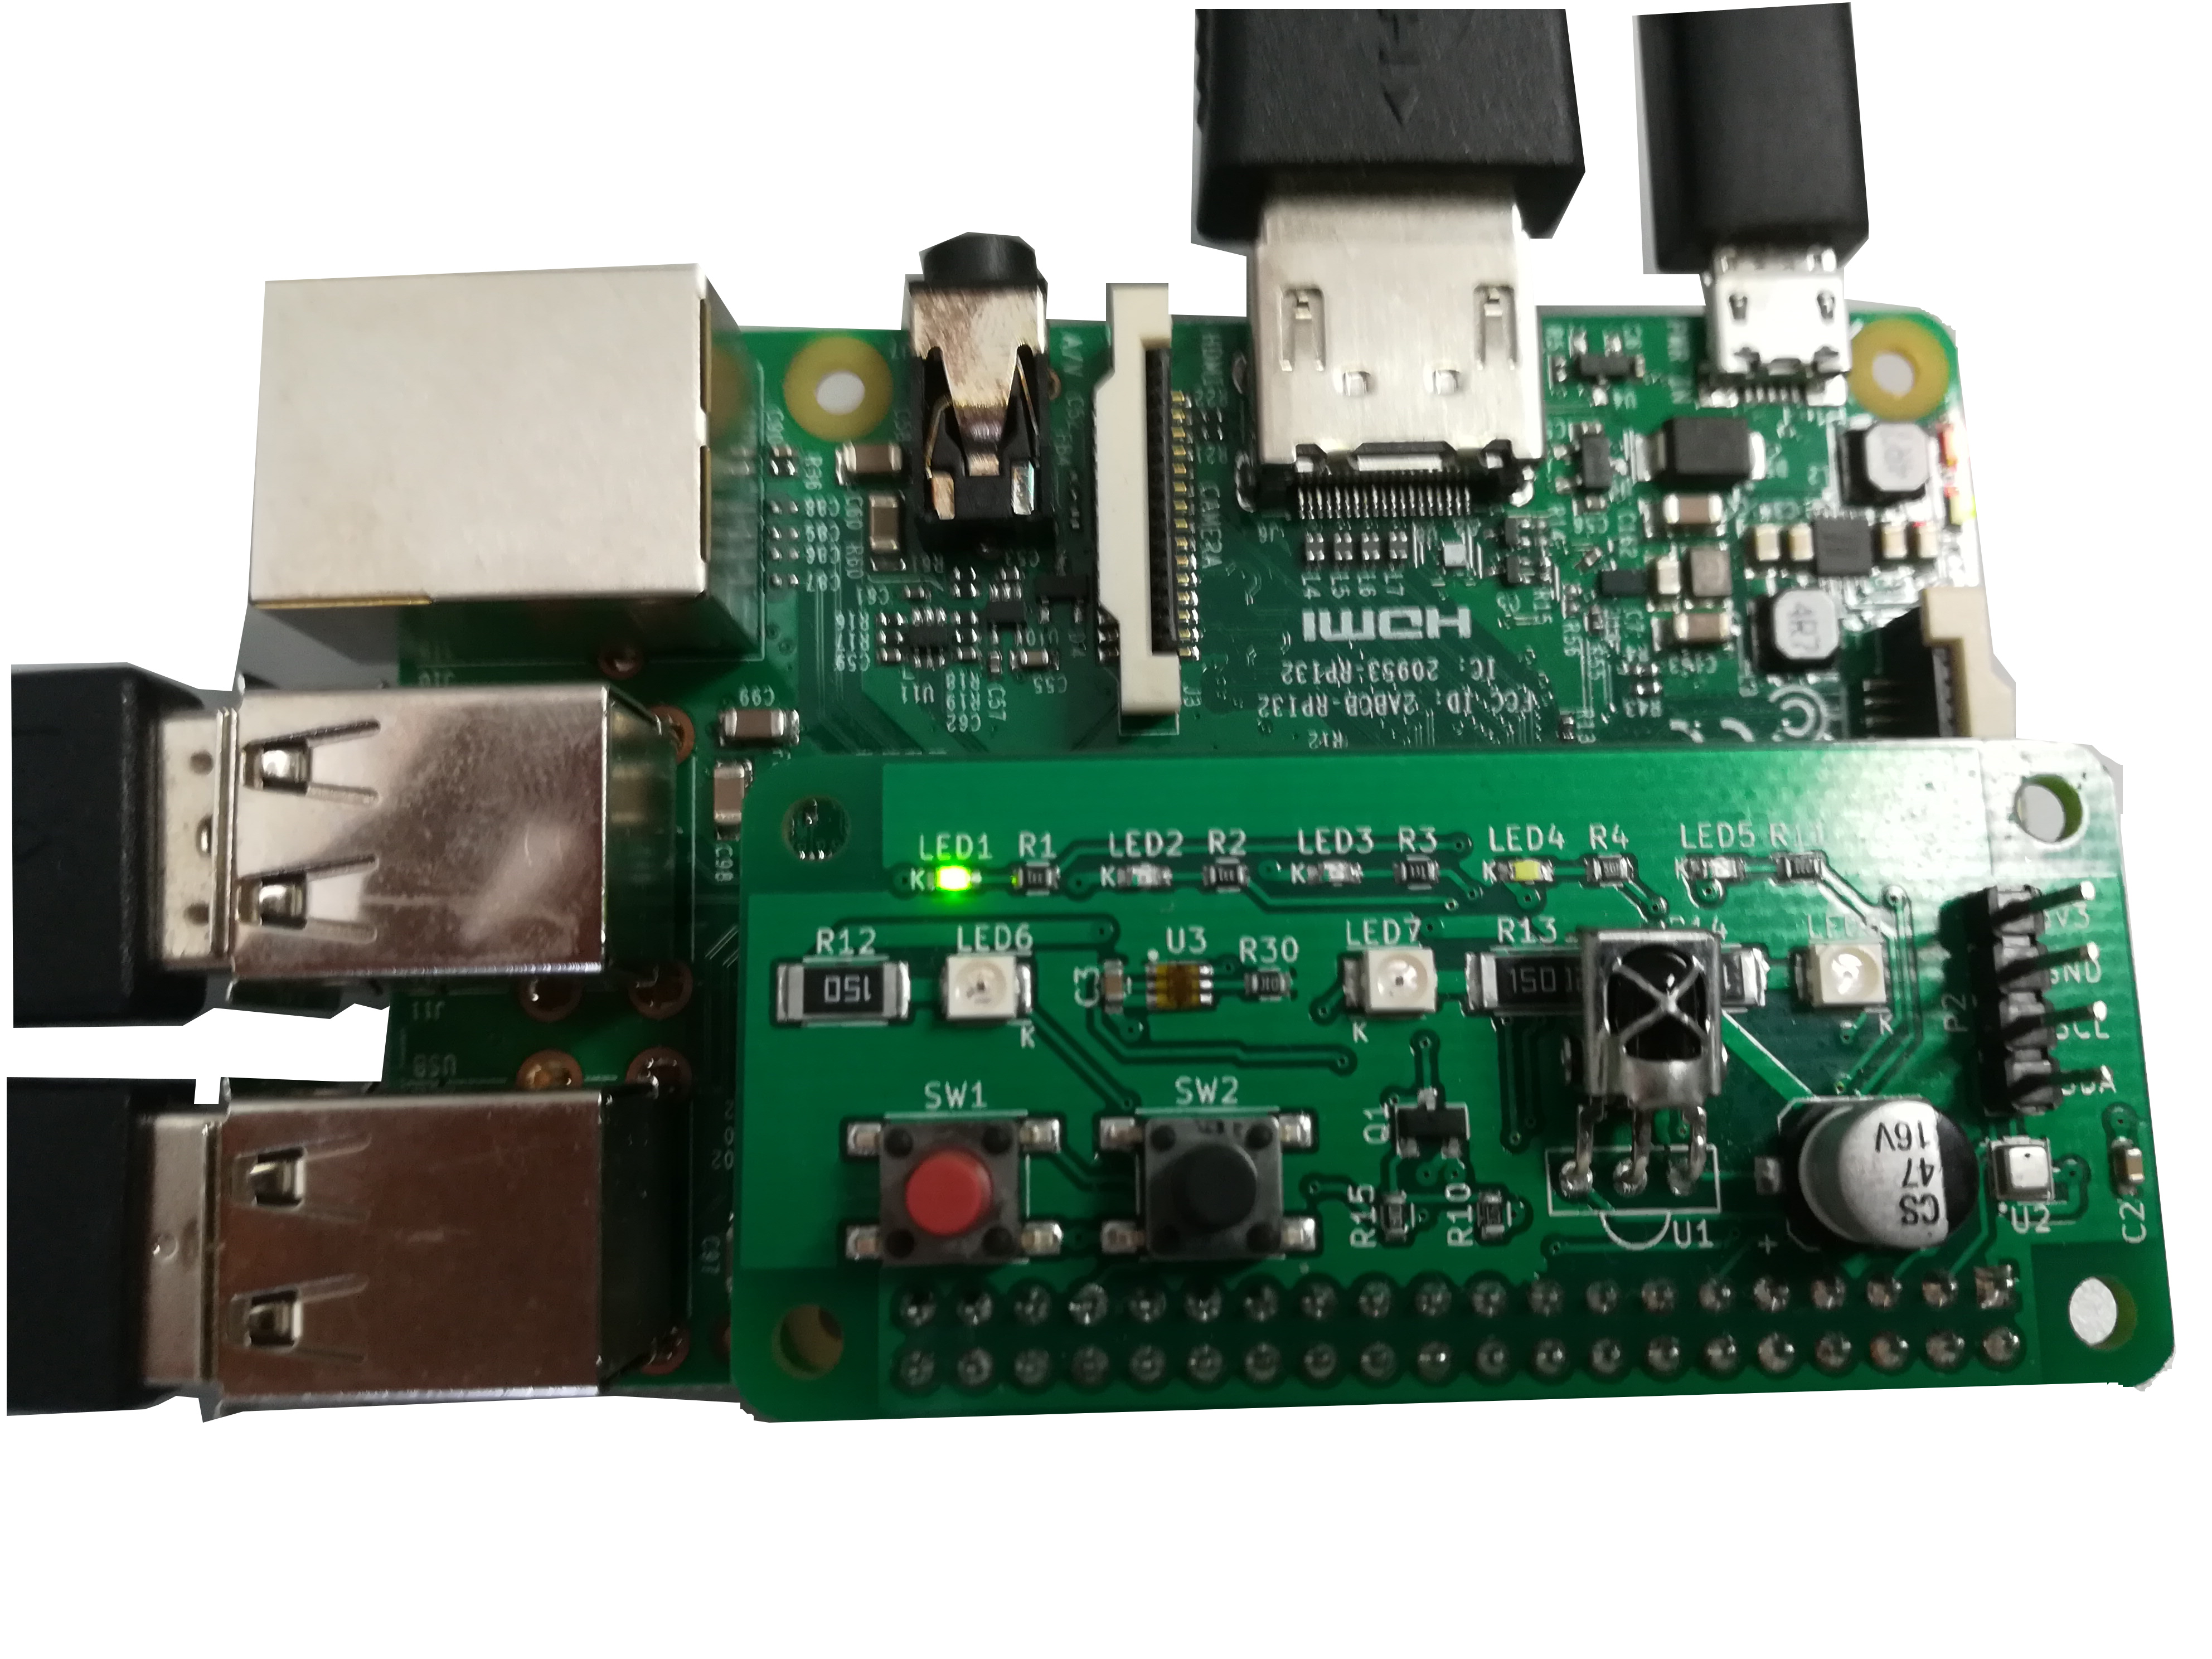
\includegraphics[width=\linewidth]{images/chap03/text03-img032.jpg}
\end{figure}

それではプログラムを解析してみましょう。\code{font} 命令や \code{pos} 命令、 \code{mes} 命令がありますね。これらがどんな命令だったかを前回の教科書を読んで復習しましょう。gpio 命令も前回勉強しました。17という数字は上の図\ref{sensors}の GPIO17 に対応していて、1 という数字は ON をあらわすのでしたね。\\

\begin{tcolorbox}[title=\useOmetoi]
\begin{enumerate}
\item LED を光らせる命令を書きましょう(ヒント: 教科書第 2 回 2-9 LED が点滅するスクリプトを参考にしましょう)。\\
\underline{答え.\hspace{0.8\linewidth}}
\item LED を消す命令を書きましょう(ヒント: 教科書第 2 回 2-9 LED が点滅するスクリプトを参考にしましょう)。\\
\underline{答え.\hspace{0.8\linewidth}}
\item ターミナルを使って led.hsp のコピーを、321.hsp という名前で作りましょう。\\
\fbox{\phantom{白}} $\leftarrow$できたらチェックしましょう。
\item 他の色の LED が光るように 321.hsp のプログラムを変えてみましょう。\\
\fbox{\phantom{白}} $\leftarrow$できたらチェックしましょう。
\end{enumerate}
\end{tcolorbox}

